\documentclass[11pt,a4paper]{article}
\usepackage[margin=18mm]{geometry}
\usepackage{amsmath,amssymb,mathtools}
\usepackage{booktabs,array,enumitem}
\usepackage[dvipsnames]{xcolor}
\usepackage{graphicx,listings,tikz,float,needspace}
\usetikzlibrary{arrows.meta,positioning}
\usepackage[most]{tcolorbox}
\usepackage{hyperref}
\hypersetup{colorlinks=true,urlcolor=MidnightBlue,linkcolor=MidnightBlue}
\setlength{\parindent}{0pt}\setlength{\parskip}{4pt}
\newcommand{\course}{PHY4605 Computational Methods in Physics}
\newcommand{\units}[1]{\,\mathrm{#1}}
\newtcolorbox{keybox}{colback=RoyalBlue!5,colframe=RoyalBlue!65!black,boxrule=.7pt,arc=2mm}
\newtcolorbox{checkbox}{colback=ForestGreen!5,colframe=ForestGreen!55!black,boxrule=.7pt,arc=2mm}
\newtcolorbox{aibox}{colback=BurntOrange!7,colframe=BurntOrange!80!black,boxrule=.7pt,arc=2mm}
\lstdefinestyle{matlabstyle}{language=Matlab,basicstyle=\ttfamily\footnotesize,keywordstyle=\color{RoyalBlue!75!black},commentstyle=\color{ForestGreen!55!black},stringstyle=\color{BurntOrange!80!black},numbers=left,numberstyle=\scriptsize\color{black!50},numbersep=5pt,frame=single,rulecolor=\color{RoyalBlue!25},backgroundcolor=\color{RoyalBlue!3},showstringspaces=false,columns=fullflexible,keepspaces=true,breaklines=true}
\begin{document}
{\large\textsc{\course}}\\[-2pt]
{\small Learning Note \textbar\ Week 4}\par\vspace{4pt}
{\LARGE\bfseries Parameter Sweeps and Graph Interpretation}\par\vspace{3pt}
\textit{Use one familiar spring model to turn parameter variation into a controlled computational experiment.}

\begin{keybox}\textbf{Physical question.} If the same forces are applied to springs with different stiffness values, how can we compare their extensions fairly and explain the trend using both the graph and Hooke's law?\end{keybox}

\section*{Core learning outcomes}
\begin{enumerate}[nosep,leftmargin=5mm]
\item design a controlled sweep that varies one physical parameter while keeping the model and other inputs fixed;
\item evaluate and overlay several parameter cases on common labelled axes; and
\item validate a known or limiting case and explain the trend in physical language.
\end{enumerate}

\section*{1. A parameter sweep is a controlled experiment}
A parameter sweep asks the \emph{same physical question} several times while deliberately changing one input parameter. The comparison is meaningful only when the equation, independent-variable array, assumptions, and all other parameters remain the same.

\begin{center}
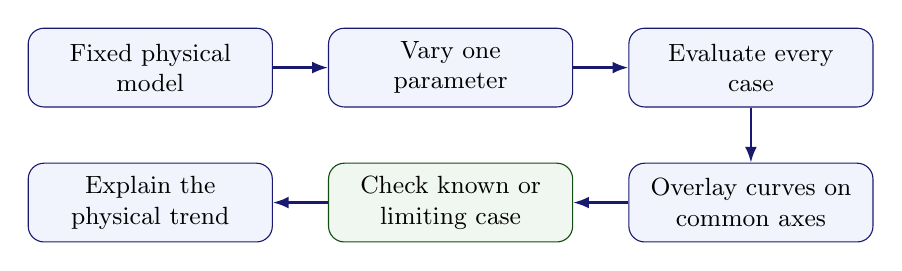
\begin{tikzpicture}[node distance=7mm and 7mm,every node/.style={font=\small,align=center},box/.style={draw=MidnightBlue,rounded corners=2mm,fill=RoyalBlue!7,minimum width=31mm,minimum height=10mm},check/.style={draw=ForestGreen!55!black,rounded corners=2mm,fill=ForestGreen!7,minimum width=31mm,minimum height=10mm},arrow/.style={-{Latex[length=2mm]},thick,MidnightBlue}]
\node[box] (model) {Fixed physical\\model};
\node[box,right=of model] (param) {Vary one\\parameter};
\node[box,right=of param] (eval) {Evaluate every\\case};
\node[box,below=of eval] (plot) {Overlay curves on\\common axes};
\node[check,left=of plot] (check) {Check known or\\limiting case};
\node[box,left=of check] (interp) {Explain the\\physical trend};
\draw[arrow] (model)--(param); \draw[arrow] (param)--(eval); \draw[arrow] (eval)--(plot); \draw[arrow] (plot)--(check); \draw[arrow] (check)--(interp);
\end{tikzpicture}
\end{center}

\begin{aibox}\textbf{Common mistake.} If two parameters change at the same time, the graph may still look smooth, but the difference between curves can no longer be attributed to one cause. That is a confounded comparison, not a controlled sweep.\end{aibox}

\section*{2. Familiar model: an ideal spring}
Within its linear elastic range, an ideal spring follows Hooke's law,
\[
F=kx,
\qquad\text{so}\qquad
x=\frac{F}{k}.
\]
In words: \emph{extension equals applied force divided by spring stiffness}. For a fixed force, increasing stiffness must reduce extension.

\begin{center}\small
\begin{tabular}{>{\raggedright\arraybackslash}p{.18\linewidth}>{\raggedright\arraybackslash}p{.23\linewidth}>{\raggedright\arraybackslash}p{.46\linewidth}}
\toprule
\textbf{Symbol} & \textbf{MATLAB name} & \textbf{Meaning and unit}\\
\midrule
$F$ & \texttt{F\_N} & applied force, N; common input array\\
$k$ & \texttt{k\_Npm} & spring stiffness, N m$^{-1}$; swept parameter\\
$x$ & \texttt{extension\_m} & spring extension, m; calculated output\\
\bottomrule
\end{tabular}
\end{center}

Use the common force array $F=0$ to $10\units{N}$ and three stiffnesses: $50$, $100$, and $200\units{N\,m^{-1}}$. Treat $100\units{N\,m^{-1}}$ as the baseline.

\begin{checkbox}\textbf{Prediction checkpoint.} At the same positive force, the $50\units{N\,m^{-1}}$ spring should extend the most and the $200\units{N\,m^{-1}}$ spring the least. At $F=0$, every ideal spring must have $x=0$.\end{checkbox}

\section*{3. Decide what changes and what stays fixed}
Before writing code, make the experimental control explicit.

\begin{center}\small
\begin{tabular}{>{\raggedright\arraybackslash}p{.30\linewidth}>{\raggedright\arraybackslash}p{.54\linewidth}}
\toprule
\textbf{Deliberately changed} & \textbf{Held fixed}\\
\midrule
Spring stiffness $k$: 50, 100, 200 N/m & Hooke model $x=F/k$, force array $0:0.5:10$ N, ideal-linear assumption, plotting axes, and output definition\\
\bottomrule
\end{tabular}
\end{center}

This control statement is part of the scientific result. It tells the reader what can legitimately explain the difference between curves.

\section*{4. Pseudocode before MATLAB}
\begin{enumerate}[nosep,leftmargin=7mm]
\item define one common applied-force array;
\item define a small array of stiffness values and identify the baseline;
\item for each stiffness, calculate $x=F/k$ using the same force values;
\item store one extension curve for each stiffness;
\item overlay all curves using the same axes and a legend;
\item compare the same force across cases;
\item check the zero-force limiting case; and
\item explain why the curves differ using the physical equation.
\end{enumerate}

\section*{5. Build a small parameter array}
The force array contains the repeated physical inputs. The stiffness array contains the cases to compare.
\begin{lstlisting}[style=matlabstyle]
F_N = 0:0.5:10;       % common applied-force array (N)
k_Npm = [50 100 200]; % swept spring stiffness values (N/m)
baseline_k_Npm = 100; % baseline case (N/m)
\end{lstlisting}
The comparison uses only three stiffness values because the goal is to make the trend visible and traceable. A dense sweep is not automatically a better experiment.

\section*{6. Evaluate the same model for every case}
Preallocate one matrix row for each stiffness. The loop changes only the selected stiffness value; the force array and equation remain unchanged.
\begin{lstlisting}[style=matlabstyle]
extension_m = zeros(length(k_Npm),length(F_N));
for case_id = 1:length(k_Npm)
    extension_m(case_id,:) = F_N./k_Npm(case_id);
end
\end{lstlisting}
Row 1 stores the $50\units{N\,m^{-1}}$ case, row 2 the baseline, and row 3 the $200\units{N\,m^{-1}}$ case. At $F=10\units{N}$,
\[
x=\frac{10}{50}=0.20\units{m},\quad
x=\frac{10}{100}=0.10\units{m},\quad
x=\frac{10}{200}=0.05\units{m}.
\]

\begin{checkbox}\textbf{Code-tracing checkpoint.} In \texttt{extension\_m(3,end)}, index 3 selects the $200\units{N\,m^{-1}}$ spring and \texttt{end} selects the largest stored force, $10\units{N}$. The expected value is $0.05\units{m}$.\end{checkbox}

\section*{7. Overlay curves so the comparison is fair}
All parameter cases should share the same axes. A legend identifies which curve belongs to which stiffness.
\begin{lstlisting}[style=matlabstyle]
plot(F_N,extension_m.','LineWidth',2)
grid on
xlabel('Applied force, F (N)')
ylabel('Spring extension, x (m)')
title('Hooke''s Law Parameter Sweep: Effect of Spring Stiffness')
legend('k = 50 N/m','k = 100 N/m','k = 200 N/m')
\end{lstlisting}

\begin{figure}[H]
\centering
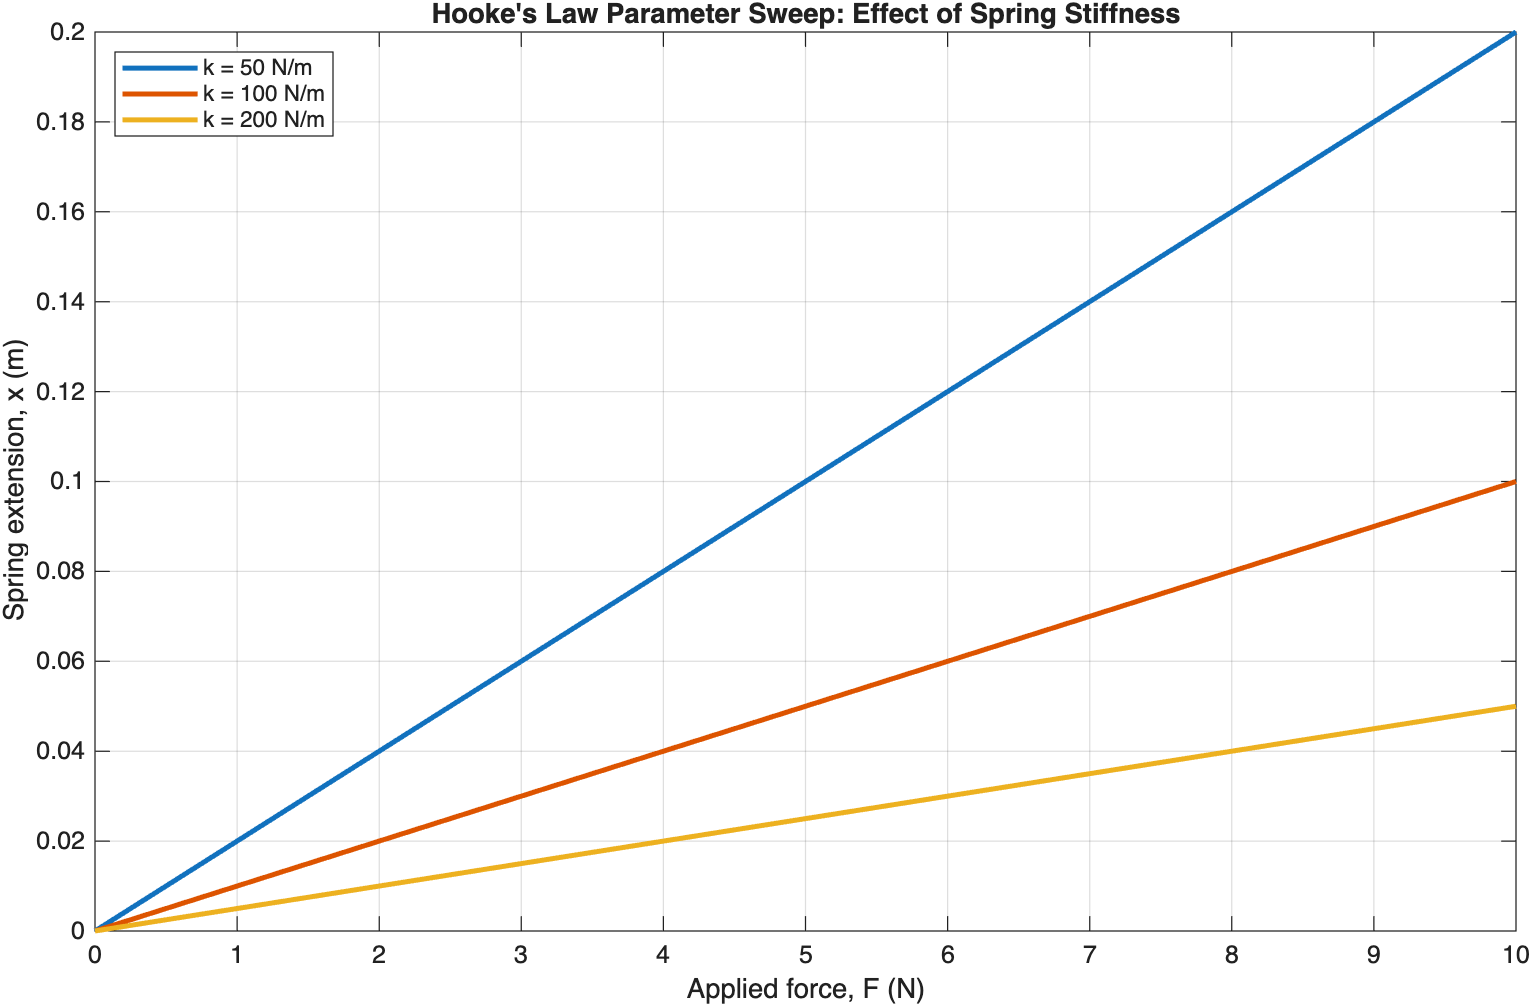
\includegraphics[width=.88\linewidth]{../matlab/assets/week04_hooke_parameter_sweep.png}
\caption{MATLAB-generated parameter sweep for the locked Hooke model. Every curve uses the same applied-force array; only spring stiffness changes.}
\end{figure}

\section*{8. Read the graph as physics, not only as geometry}
The three curves are straight because $x$ is proportional to $F$ when $k$ is fixed. Their slopes differ because the slope is $1/k$. A smaller stiffness gives a larger slope, so the spring extends more for each additional newton of force. A larger stiffness gives a smaller slope, so the same load produces less deformation.

\begin{keybox}\textbf{Graph interpretation rule.} Do not stop at ``the blue line is steeper.'' State the physical cause: the smaller stiffness produces more extension at the same force because $x=F/k$.\end{keybox}

\section*{9. Core validation: zero-force limiting case}
At zero applied force,
\[
x(0)=\frac{0}{k}=0
\]
for every positive stiffness. This check is known before running the program and tests all swept cases simultaneously.
\begin{lstlisting}[style=matlabstyle]
zero_force_extension_m = extension_m(:,1);
assert(max(abs(zero_force_extension_m)) < 1e-12,...
    'Zero-force limiting-case validation failed.')
\end{lstlisting}
\begin{checkbox}\textbf{Validation result.} The first stored extension is 0 m for all three stiffness values, so the limiting case passes from a fresh MATLAB session.\end{checkbox}

\section*{10. Diagnose a runnable but physically wrong model}
Suppose the model is entered as \texttt{x = F.*k}. MATLAB can calculate that expression, but it no longer represents Hooke's law. The units are wrong and the trend reverses: larger stiffness would produce a larger numerical output.

\begin{center}\small
\begin{tabular}{>{\raggedright\arraybackslash}p{.27\linewidth}>{\raggedright\arraybackslash}p{.30\linewidth}>{\raggedright\arraybackslash}p{.29\linewidth}}
\toprule
\textbf{Check} & \textbf{Correct $x=F/k$} & \textbf{Wrong $F\,k$}\\
\midrule
Units & N /(N/m) = m & N(N/m), not m\\
Stiffness trend & larger $k$ gives smaller $x$ & larger $k$ gives larger value\\
At $F=0$ & zero & also zero; this check alone cannot expose the formula error\\
\bottomrule
\end{tabular}
\end{center}

\begin{aibox}\textbf{Responsible-AI caution.} A generated script can pass one limiting-case check and still encode the wrong equation. Use several kinds of evidence together: physical model, units, expected trend, and the selected validation check.\end{aibox}

\section*{Working exposure: selected values and a two-parameter table}
Selected-value tables can compare exact outputs at a few common forces. A supplied two-parameter table may broaden the comparison, but designing heatmaps is not Core Week 4 work.

\section*{Optional stretch: local sensitivity}
At fixed force, $\partial x/\partial k=-F/k^2$. The negative sign formalises the Core trend: increasing stiffness reduces extension. Quantitative sensitivity is not required for the Week 4 pass-level route.

\section*{Three takeaways}
\begin{enumerate}[nosep,leftmargin=6mm]
\item A controlled parameter sweep changes one named parameter while keeping the model and other inputs fixed.
\item Overlay curves on common labelled axes and compare the same physical input across cases.
\item Explain the trend using the physical equation, then validate at least one known or limiting case before trusting the result.
\end{enumerate}

\begin{keybox}\textbf{Preparation for the practical.} Be ready to transfer the same sweep logic to Ohm's law, vertical motion, and a small-angle pendulum. For every context, state what changes, what stays fixed, what the graph should show, and which independent check makes the comparison credible.\end{keybox}
\end{document}
